\documentclass[tikz,border=10pt]{standalone}
% Shared look for every TikZ diagram. Load with \input{../../tools/tikz-style.tex}
\usepackage[T1]{fontenc}
\usepackage{lmodern}
\renewcommand{\sfdefault}{lmr}  % diagrams use the same serif as the text
\usetikzlibrary{arrows.meta, positioning, shapes.geometric, calc, fit, backgrounds}
\definecolor{cblue}{HTML}{4C78A8}
\definecolor{corange}{HTML}{F58518}
\definecolor{cgreen}{HTML}{54A24B}
\definecolor{cred}{HTML}{E45756}
\definecolor{cpurple}{HTML}{B279A2}
\definecolor{cgrey}{HTML}{6B6B6B}
\tikzset{
  every picture/.style={font=\sffamily, line width=1.2pt},
  box/.style={draw=#1, fill=#1!12, rounded corners=4pt, align=center, inner sep=7pt, minimum height=1.1cm},
  box/.default=cgrey,
  arrow/.style={-{Stealth[length=3mm]}, draw=cgrey, line width=1.4pt},
  title/.style={font=\sffamily\bfseries\Large},
  note/.style={font=\sffamily\small, text=cgrey, align=center},
}
\AtBeginDocument{\hyphenpenalty=10000 \exhyphenpenalty=10000}

\begin{document}
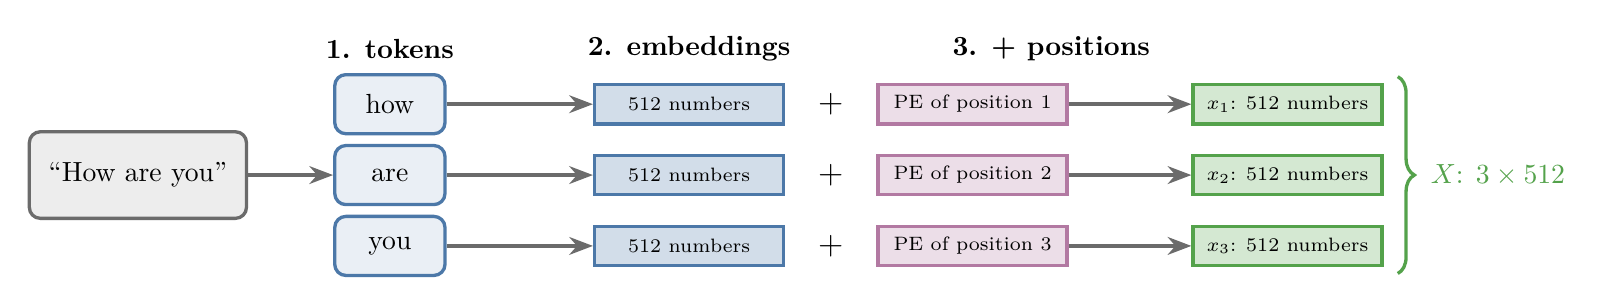
\begin{tikzpicture}[t/.style={box=cblue, minimum width=1.4cm, minimum height=0.75cm, font=\sffamily},
  v/.style={draw=#1, fill=#1!25, minimum width=2.4cm, minimum height=0.5cm, inner sep=1pt, font=\sffamily\scriptsize}]
  \node[box=cgrey, font=\sffamily] (s) at (0,0) {``How are you''};
  \node[font=\sffamily\bfseries] at (3.2,1.6) {1. tokens};
  \node[font=\sffamily\bfseries] at (7.0,1.6) {2. embeddings};
  \node[font=\sffamily\bfseries] at (11.6,1.6) {3. + positions};
  \foreach \w/\y [count=\k] in {how/0.9, are/0, you/-0.9} {
    \node[t] (t\k) at (3.2,\y) {\w};
    \node[v=cblue] (e\k) at (7.0,\y) {512 numbers};
    \node[v=cpurple] (p\k) at (10.6,\y) {PE of position \k};
    \node[font=\sffamily\large] at (8.8,\y) {$+$};
    \node[v=cgreen] (x\k) at (14.6,\y) {$x_\k$: 512 numbers};
    \draw[arrow] (t\k) -- (e\k);
    \draw[arrow] (p\k) -- (x\k);
  }
  \draw[arrow] (s) -- (t2);
  \draw[decorate, decoration={brace, amplitude=6pt}, cgreen] (16.0,1.25) -- node[right=8pt, font=\sffamily, text=cgreen] {$X$: $3 \times 512$} (16.0,-1.25);
\end{tikzpicture}
\end{document}
